\documentclass[17pt, orivec]{extarticle} % 12pt, 14pt, 17pt, 20pt
\usepackage{amsmath}
\usepackage{amssymb}    % for \rightsquigarrow
\usepackage{wasysym}	% for frown face
\usepackage{mathrsfs} 	% for \mathscr
\usepackage{stmaryrd}
\usepackage[most]{tcolorbox}
\usepackage{ulem}
\usepackage{tikz-cd}		% commutative diagrams
\usepackage{tikz}
\usepackage{amsthm}
\usepackage{enumitem}	% for \itemize custom labels
\usepackage{turnstile}	% longer turnstiles
\usepackage[sf,bf,big,raggedright,compact]{titlesec}	% change section color to blue
% \usepackage[backend=biber,bibstyle=authoryear,citestyle=../authoryearbrack]{biblatex}
% \bibliography{../AGI-book}

\newtheorem{theorem}{Theorem}

\ifdefined\chinchin
	\newcommand{\cc}[2]{#1}
	\usepackage[CJKspace]{xeCJK}
	%\setCJKmainfont[BoldFont=SimHei,ItalicFont=AR PL KaitiM GB]{Alibaba PuHuiTi}
	\setCJKmainfont[BoldFont=Alibaba-PuHuiTi-Regular.ttf, ItalicFont=gkai00mp.ttf]{Alibaba-PuHuiTi-Light.ttf}
	% \setmainfont[ItalicFont=Latin Modern Roman Slanted]{Alibaba Sans:style=Light}
\else
	\newcommand{\cc}[2]{#2}
	% \setmainfont[ItalicFont=Latin Modern Roman Slanted]{Alibaba Sans:style=Light}
	%\renewcommand{\baselinestretch}{0.8} 
\fi

%\ifdefined\chinchin
%\newcommand{\cc}[2]{#1}
%\usepackage[CJKspace]{xeCJK}
%\setCJKmainfont[BoldFont=SimHei,ItalicFont=AR PL KaitiM GB]{SimSun}
%\else
%\newcommand{\cc}[2]{#2}
%\fi

\setlength{\headheight}{0cm}
\setlength{\hoffset}{0cm}
\setlength{\topmargin}{-2cm}
\setlength{\oddsidemargin}{-2cm}
\setlength{\evensidemargin}{-2cm}
\setlength{\textwidth}{20cm}
\setlength{\textheight}{26cm}
\setlength{\headsep}{0cm}
\setlength{\topskip}{0cm}
\setlength{\footskip}{0.9cm}  % between bottom of page and page number
\setlength{\floatsep}{0cm}
\setlength{\textfloatsep}{0.6cm}
\setlength{\intextsep}{0.5cm}
\setlength{\parindent}{0em}   % em = width of capital M

% Fix spilling of titles in bibliography:
%\DeclareFieldFormat*{title}{#1}
%
%\DeclareFieldFormat*{titlecase}{%
%    \ifdef{\currentfield}
%      {\ifcurrentfield{title}
%         {\usefield{\uline}{\currentfield}}%
%         {#1}}
%      {#1}}

\setcounter{secnumdepth}{2}		% no section numbers

\titleformat{\section}[hang]{\bfseries\Large\color{blue}}{\thesection \hspace{20pt}}{0pt}{}
\titleformat{\subsection}[hang]{\bfseries\large\color{blue}}{\thesubsection \hspace{10pt}}{0pt}{}
\titleformat{\subsubsection}[hang]{\bfseries\color{blue}}{}{0pt}{}

\itemsep0em
\setlist[itemize]{noitemsep, topsep=-5pt, partopsep=-5pt}
\renewcommand{\labelitemi}{$\textbullet$}

\let\varzero\emptyset
\let\emptyset\varnothing		% round empty set 
\newcommand{\vect}[1]{\boldsymbol{#1}}
\newcommand{\book}[1]{$\NewSym[0.4]{../book-icon.png} \quad$ \parbox{0.9\textwidth}{\footnotesize #1}}
\newcommand{\code}[1]{{\footnotesize{\ttfamily #1}}}
\newcommand{\tab}{\hspace*{2cm}}
\newcommand{\powerset}{\raisebox{.15\baselineskip}{\Large\ensuremath{\wp}}}
\newcommand{\Chi}{\raisebox{2.5pt}{$\chi$}}
\newcommand*\KB{\vcenter{\hbox{
\includegraphics{../KB-symbol.png}}}}
\newcommand*\NewSym[2][0.5]{\vcenter{\hbox{\includegraphics[scale=#1]{#2}}}}
\newcommand*\sigmoid{\vcenter{\hbox{
\includegraphics{../sigmoid3.png}}}}
\newcommand{\smbox}[1]{\boxed{\footnotesize{\mbox{#1}}}}

\newcommand{\tikzmark}[1]{\tikz[overlay,remember picture] \node (#1) {};}

\newcommand{\Dfrac}[2]{%
\ooalign{%
      $\genfrac{}{}{2.9pt}0{\hphantom{#1}}{\hphantom{#2}}$\cr%
      $\color{white}\genfrac{}{}{1.5pt}0{\hphantom{#1}}{\hphantom{#2}}$\cr%
      $\color{white}\genfrac{}{}{1pt}0{\color{black}#1}{\color{black}#2}$}}

% \renewcommand{\thefootnote}{\fnsymbol{footnote}}
\usepackage{perpage}
\MakePerPage{footnote}
\renewcommand{\thefootnote}{\ifcase\value{footnote}\or{*}
	\or{$\dagger$}\or{**}\or{$\ddagger$}\fi}
\interfootnotelinepenalty=10000

\setlength{\parindent}{0pt}
\setlength{\parskip}{1.8ex plus0.8ex minus0.8ex}

% \usepackage[no-math]{fontspec}
% \setmainfont[BoldFont=Alibaba_Sans_Regular.otf,ItalicFont=Alibaba_Sans_Light_Italic.otf]{Alibaba_Sans_Light.otf}

\usepackage[backend=biber]{biblatex}
\bibliography{../AGI-book}

% \usepackage[active,tightpage]{preview}		% for continuous page(s)
% \renewcommand{\PreviewBorder}{0.5cm}
% \renewcommand{\thempfootnote}{\arabic{mpfootnote}}

% \usepackage[absolute,overlay]{textpos}		% for page number on upper left corner

\usepackage{color}
% \usepackage{mathtools}
\usepackage[hyperfootnotes=false]{hyperref}
\usepackage{enumitem}
\setlist[itemize]{noitemsep, topsep=0pt}

% \usepackage[backend=biber,style=numeric]{biblatex}
% \bibliography{../AGI-book}
% \renewcommand*{\bibfont}{\footnotesize}

\usetikzlibrary{shapes}
% \usepackage[export]{adjustbox}	% ??
\usepackage{verbatim} % for comments
% \usepackage{newtxtext,newtxmath}	% Times New Roman font

% \titleformat{\section}[hang]{\bfseries\large\color{blue}}{}{0pt}{}
% \numberwithin{equation}{subsection}

\newcommand{\underdash}[1]{%
	\tikz[baseline=(toUnderline.base)]{
		\node[inner sep=1pt,outer sep=10pt] (toUnderline) {#1};
		\draw[dashed] ([yshift=-0pt]toUnderline.south west) -- ([yshift=-0pt]toUnderline.south east);
	}%
}%

\newcommand\reduline{\bgroup\markoverwith{\textcolor{red}{\rule[-0.5ex]{2pt}{0.4pt}}}\ULon}

%\DeclareSymbolFont{symbolsC}{U}{txsyc}{m}{n}
%\DeclareMathSymbol{\strictif}{\mathrel}{symbolsC}{74}
%\DeclareSymbolFont{AMSb}{U}{msb}{m}{n}
%\DeclareSymbolFontAlphabet{\mathbb}{AMSb}
%\setmathfont{lmroman17-regular.otf}
\DeclareMathOperator*{\argmin}{arg\,min}
\DeclareMathOperator*{\argmax}{arg\,max}

% \usepackage[most]{tcolorbox}
%\tcbset{on line,
%	boxsep=4pt, left=0pt,right=0pt,top=0pt,bottom=0pt,
%	colframe=red,colback=pink,
%	highlight math style={enhanced}
%}
%\newcommand{\atom}{\vcenter{\hbox{\tcbox{....}}}}

\let\oldtextbf\textbf
\renewcommand{\textbf}[1]{\textcolor{cyan}{\oldtextbf{#1}}}

\newcommand{\logic}[1]{{\color{violet}{\textit{#1}}}}
\newcommand{\underconst}{
\includegraphics[scale=0.5]{../2020/UnderConst.png}}
\newcommand{\KBsymbol}{\vcenter{\hbox{
\includegraphics[scale=1]{../KB-symbol.png}}}}
\newcommand{\token}{\vcenter{\hbox{\includegraphics[scale=1]{token.png}}}}
\newcommand{\proposition}{\vcenter{\hbox{\includegraphics[scale=0.8]{proposition.png}}}}
\newcommand{\defeq}{\mathrel{:}=}

\begin{document}

\cc{
\title{
	\centerline{
\includegraphics[scale=0.5]{凝聚力-logo-0.png}}
	\vspace{-0.5cm} \bfseries\color{cyan}{\Large Solidi 加密貨幣 - 白皮書}}
}{
\title{
	\centerline{
\includegraphics[scale=0.4]{Solidarity-logo-0.png}}
	\vspace{-0.5cm} \bfseries\color{cyan}{\LARGE Solidi Coin - White Paper}}
}

% \cc{
% \author{YKY (甄景賢)}}{
% \author{YKY (Yan King Yin)}
% }

\date{\vspace{-1.8cm}{\small \today}} % Date, can be changed to a custom date

\maketitle

\setcounter{section}{0}
\newcounter{mypage}
\setcounter{mypage}{0}

% (1) Circled page number on upper left corner
%\begin{textblock*}{5cm}(2.1cm,2.3cm) % {block width} (coords)
%{\color{red}{\large \textcircled{\small \themypage}}}
%\addtocounter{mypage}{1}
%\end{textblock*}

\section{\cc{Solidi 的貨幣經濟學}{Economics of the Solidi Coin}}

\begin{itemize}
\cc{
	\item Solidi 幣的特點 是以\textbf{投票}形式 賺取的,例如 在新聞平台上發評論,被 \textbf{點贊} 即能獲得 貨幣獎勵:
	\begin{equation}
		\nonumber
		\vcenter{\hbox{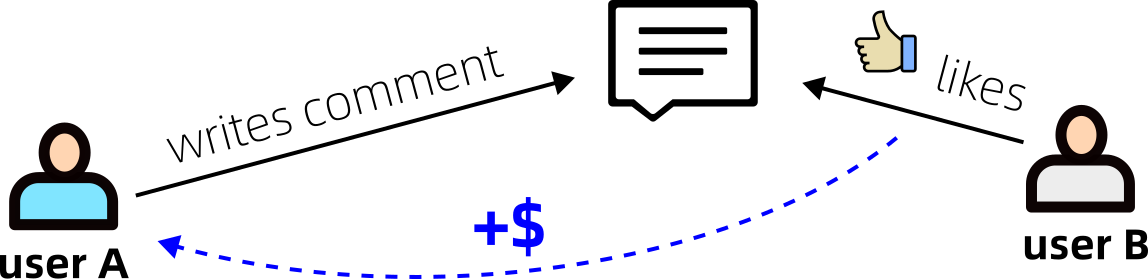
\includegraphics[scale=0.5]{likes-equal-coins.png}}}
	\end{equation}
	幣值也稱爲 \textbf{聲譽},也等於 \textbf{投票權} (下述)。
}{
	\item Solidi coins are earned via \textbf{voting}.  For example, if your comment on a news site is liked by someone, you get rewarded with Solidi:
	\begin{equation}
		\nonumber
		\vcenter{\hbox{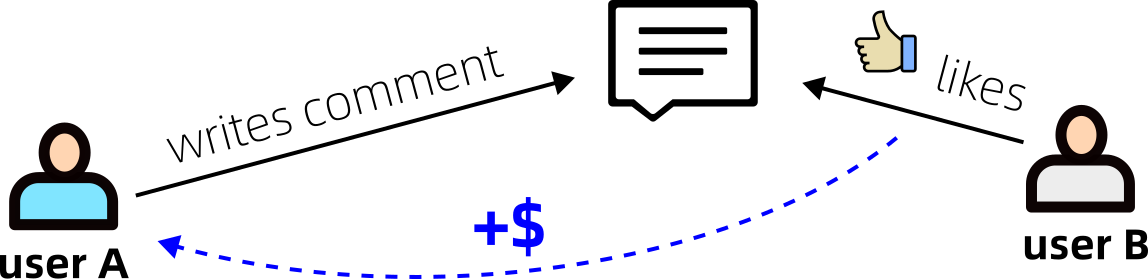
\includegraphics[scale=0.5]{likes-equal-coins.png}}}
	\end{equation}
	Coins are also synonymous with \textbf{Reputation}, and also equivalent to \textbf{Voting Power} (explained below).
}

\cc{
	\item \textbf{指數式 兌換:}  用戶可以花錢買 聲譽/投票權,但所需的價錢 會隨着聲譽 \textbf{指數式}增加。 換句話說,即使最有錢的個人或基金,都無法用錢換取極大的聲譽值,這保障了 聲譽不會純粹被 資本 主導。也可以說 Solidi 跟現時世界上的 money 是不同類的一種價值,它可以糾正 貧富懸殊的 財富分配,因爲現時世界的財富分配 服從 log-normal distribution (對數-正態分佈)。\footnote{譬如《正義》一書的作者、哈佛大學教授 Michael Sandel 說: 大部分人都很感激我們的中學、小學老師,而我們也欣賞 美斯 (Lionel Messi) 的世界足球技藝,但 美斯 的薪金 卻是一般教師薪金 的接近 1,000 倍,令人質疑社會制度是否出了問題? \\ 至於爲什麼 財富呈現 對數式分佈? 數學上這是出於某種「乘法」的效應,但確切來說我不太清楚這乘法的解釋。 或者一個例子是:在菜市場,人們不會買「平均」的蘋果,而是選擇最好的蘋果,剩下的爛蘋果沒人要。 或許是這種機制導致「貧者愈貧、富者愈富」?} 以下說「現金」泛指傳統金錢。
}{
	\item \textbf{Exponential Conversion.}  A member can spend money to ``pump up'' his reputation, but it gets \textbf{exponentially} more expensive as his reputation goes up.  % $e^{kR}$ is required to increase one unit of $R$, where $R$ is reputation, $k$ is a scaling constant, eg. $1/1000$.
	This prevents reputation from being dominated solely by capital, as even the wealthiest individuals or funds could not buy a lot of reputation.  In other words, Solidi is essentially different from traditional money;  It may correct the problem of unfair wealth distribution\footnote{As Michael Sandel, Harvard professor and author of the book ``Justice,'' says:  most of us are grateful to our high school teachers, and we also admire the soccer skills of Lionel Messi, but Messi's salary is nearly a thousand times that of a school teacher's, making us question that something may be wrong with our society.}, as current wealth in our world follows a log-normal distribution.  Below, ``money'' or ``cash'' refers to traditional money.
}

\cc{
	\item \textbf{提取款項:}  用 Solidi 兌換現金, 即上述的逆運算,則可以得到對數式的現金值。但這樣,當某會員得到了稍為可觀的聲譽,就很有可能 cash-out (withdraw),獲得現金,而導致平台因缺乏現金而崩盤。 解決辦法是: cash-out 是根據 整體 聲譽的 \textbf{比例} 計算的。 當現金儲備 (即傳統 money) 很少的時候,cash-out 微不足道。 用一句口號概括就是:「指數式買入、線性賣出」
}{
	\item \textbf{Withdrawal} is the reverse of the above, but this may be problematic.  As some users get considerable reputation, they may be tempted to cash-out (withdraw), causing the platform to run out of cash and collapse.  How to prevent this?  A solution is to calculate withdrawal as a \textbf{proportion} of the cash pool.  This means that when the total cash reserve of the platform is low, withdrawals are also insignificant.  In slogan this may be summarized as: \textit{buy exponentially, sell proportionately}.
}

\cc{
	\item \textbf{「點贊」的慷概性:}  賺取 聲譽 是很容易的,例如,每次 ``like'' 別人的評論,則評論者獲得 +1 聲譽值,而點贊者 扣除 $\frac{1}{100}$ 聲譽值。 因此人們不會吝嗇 給別人點贊。
}{
	\item \textbf{Generosity of Likes.}  Every time a member likes a comment, the creator of the comment get +1 unit reputation, while the sender gets $\frac{1}{100}$ deduction in reputation.  This encourages users not to be stingy with likes.
}

\cc{
	\item 我們的 \textbf{核心價值} 是:
	\begin{equation} \nonumber
		\vcenter{\hbox{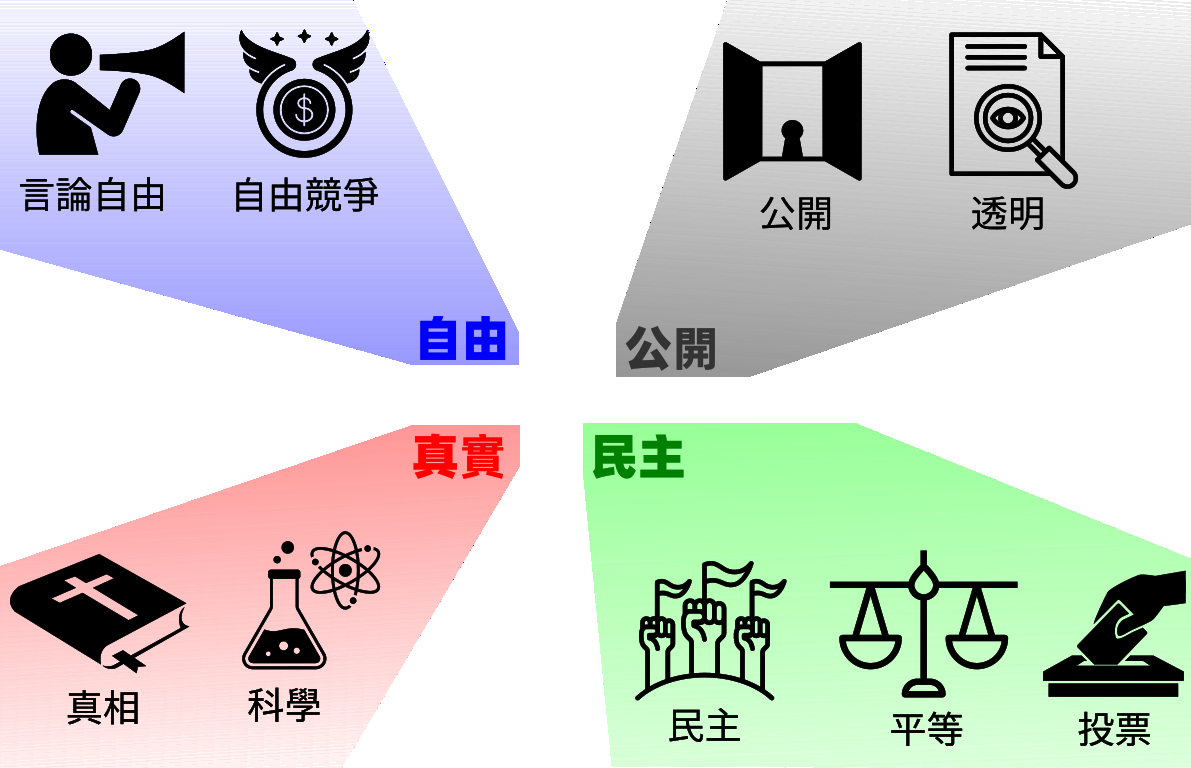
\includegraphics[scale=0.7]{DAO-核心價值.png}}}
	\end{equation}
	這些都是很經典的價值,在世界各地的文化裏都有其雛形,但在西方 啓蒙時代 系統性地提出,這並不表示盲目崇拜西方思想。 隨着科技進步,以上這些原則都是 \textbf{可驗證的} (verifiable),例如 區塊鏈、開源軟件 等都是可驗證的。
}{
	\item Our \textbf{Core Values} are:
	\begin{equation} \nonumber
		\vcenter{\hbox{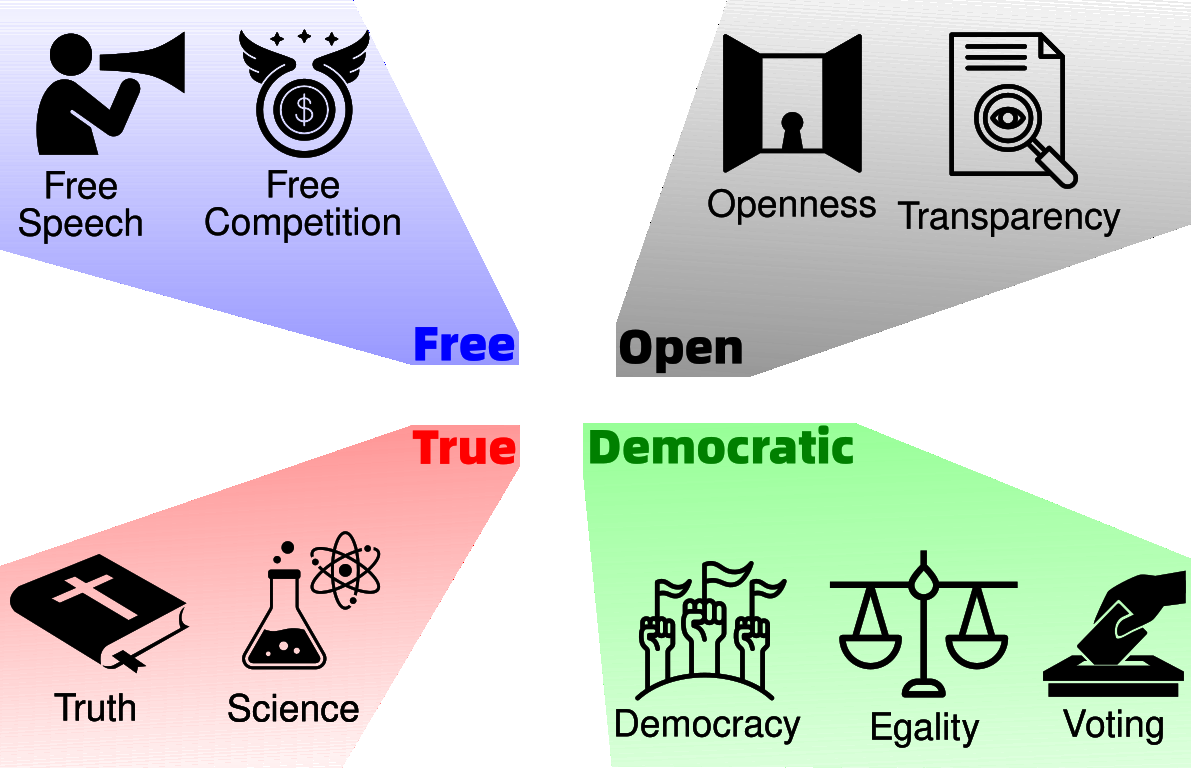
\includegraphics[scale=0.7]{DAO-principles.png}}}
	\end{equation}
	These are all very classical ideas developed in the Enlightenment period in the West, but are increasingly promoted as ``universal'' as they have primitive roots in almost every culture.  It does not mean imposing Western values on the rest of the world.  As our technology progresses, all these notions can now be \textbf{verifiable}, eg. blockchains and open-source.
}

\cc{
	\item \textbf{聲譽 有什麼價值?} 某個領域的專家,在別的領域不一定是專家,所以「聲譽」必需以不同的 領域 劃分。 我們希望 Solidi 平台完全是由 民主 的方式運行的,也就是說,以 \textbf{加權投票} 決定平台的發展方向,而 權重 就是聲譽值。 但 投票權 並不僅限於 Solidi 平台, 它可以發展到 任何領域,包括: 商業、科技、政治活動 (political activism).  很多人不明白 爲什麼 賺錢 要牽涉政治,其實在所有發展中國家(例如在非洲),不完善的政治 institutions 是 阻礙 經濟發展的主要原因,包括各種 \textbf{貪腐},導致經濟 停滯不前 甚至倒退。 後發展的人民必需改變政治制度,而 Solidi 平台是爲 全世界的 後發展國家 邁出的一步。
}{
	\item \textbf{What is the economic value of Reputation?}  Expertise in one domain does not imply it in other domains;  so Reputation should be classified by domain.  We intend the Solidi platform to operate strictly by democracy, ie. via \textbf{weighted voting} where weights are reputation.  But Reputation need not be confined to the Solidi platform;  it extends to other domains such as:  business, technology, and political activism.  Many people don't understand why business should involve politics, but the lack of well-functioning political institutions in developing countries (eg. in Africa) is a major obstacle to their economic development.  This includes various forms of \textbf{corruption}.  The people of developing nations must strive to reform our political institutions, and Solidi is a step towards this direction.
}
\end{itemize}

\section{\cc{具體細節}{Implementation details}}

\cc{
希望大家不要被數學「嚇窒」,如果懂得「指數」和「對數」是什麼,則以下只是 exp 和 log 的一些 加加減減,和 common sense 而已。 重點是: 由於「點贊的慷概性」,Solidi 的數目會快速增加,而如果增加之後 立即兌換成現金,則平台顯然會崩盤。 所以,提款時按照平台 實際有的資金,按 \textbf{比例} 結算。 那麼,即使所有人都提取 Solidi,則平台的資金復歸於 0,也沒有崩盤的問題。}{}
\begin{itemize}
	\item \textbf{Base Formula.}  To keep things simple, when a user owns $D$ Solidi coins, the equivalent amount in traditional money is \textit{defined} to be:
		\begin{equation}
			\label{eqn:base-formula}
			M \defeq M(D) \defeq e^{\frac{1}{k} \cdot D}
		\end{equation}
	where $k$ is a conversion constant to be explained in the next section.  Conversely,
		\begin{equation}
			\label{eqn:base-formula-inverse}
			D \defeq D(M) \defeq k \cdot \log M .
		\end{equation}
	The buying and selling (withdrawal) of Solidi should always refer to this formula, but withdrawal is calculated differently.

	\item \textbf{To buy} $\Delta D$ Solidi with cash $\Delta M$, when the user's current Solidi value $= D_0$.  Let $D_1 = D_0 + \Delta D$, let $M_0$ and $M_1$ be the money value corresponding to $D_0$ and $D_1$, so $M_1 = M_0 + \Delta M$.  According to the base formula, $M_0 = e^{\frac{1}{k} D_0}$.  This fixes the result:
 		\begin{eqnarray}
			\Delta D &=& D_1 - D_0 = D(M_1) - D_0 \nonumber \\
			&=& D( M_0 + \Delta M) - D_0 \nonumber \\
			&=& D( M(D_0) + \Delta M) - D_0 \nonumber \\
			&=& k \cdot \log (e^{\frac{1}{k} D_0} + \Delta M) - D_0 .
		\end{eqnarray}

	\item \textbf{To sell} $\Delta D$ Solidi, when user's current Solidi value $= D_0$, withdrawing money $\Delta M$.  Using same style of reasoning as above, we get:
 		\begin{eqnarray}
 			\label{eqn:naive-withdrawal}
			\Delta M &=& M_0 - M_1 = M(D_0) - M(D_1) \nonumber \\
			&=& M(D_0) - M(D_0 - \Delta D) \nonumber \\
			&=& e^{\frac{1}{k} D_0} + e^{\frac{1}{k} (D_0 - \Delta D)}
		\end{eqnarray}
	but this is still problematic as explained in \S1. \\
	Let the actual amount of money in the Solidi platform be $M_{Actual}$. \\
	Suppose after a lot of ``liking'' interactions, the platform has a total of $D_{Virtual}$ Solidi;  this corresponds to an amount of money:
	\begin{equation}
		M_{Virtual} = e^{\frac{1}{k} \cdot D_{Virtual}} .
	\end{equation}
	We expect that $M_{Actual} \ll M_{Virtual}$ significantly, due to the ``generosity of likes''. \\
	We cannot simply let the user withdraw $\Delta M$ as in (\ref{eqn:naive-withdrawal}), as $D_0$ and $D_1$ are based on $D_{Virtual}$, and doing so may eventually bankrupt the platform.  The solution is to pay the user \textit{proportionately} with:
	\begin{equation}
		\frac{M_{Actual}}{M_{Virtual}} \Delta M ,
	\end{equation}
	where $\Delta M$ is given by (\ref{eqn:naive-withdrawal}).

%	% This old formula used the ratio of Solidis:
%	\begin{equation}
%		W = e^{\frac{1}{k} \cdot m \frac{n}{N}} .
%	\end{equation}

\end{itemize}

\section{\cc{如何決定 常數 $k$ 的值?}{How to determine the constant $k$ ?}}

\cc{下圖 清楚顯示 Solidi 與 現金 的兌換關係,及 常數 $k$ 是如何影響 兌換。 注意: 在垂直的 $y$ 軸上,「我」和 Elon Musk 的距離並不算很遠; 但水平的 $x$ 軸是 log-scale 的,如果以正常距離計算,則 Elon 的位置已遠遠超出了熒幕的範圍、超出了我的房子、超出了香港、而到達大約 汕頭市 的位置(香港到廈門一半的距離)。
}{
Below is a log-scale plot that shows clearly how the constant $k$ affects the conversion from traditional money to Solidi coins:}
\begin{equation}
	% \vcenter{\hbox{\includegraphics[trim={0 0 0 1.5cm}, clip, scale=0.6]
	\vcenter{\hbox{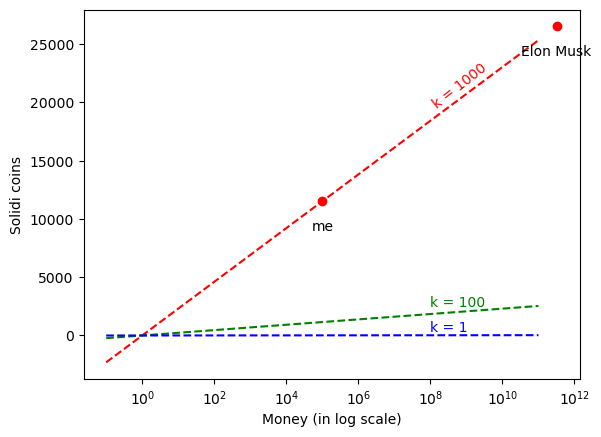
\includegraphics[scale=0.75] {Solidi-plot.png}}}
	\label{fig:log-scale-money-vs-Solidi}
	% \caption{showing how different values of $k$ affect conversion between money and Solidi.}
\end{equation}

\cc{
其中一個決定 $k$ 的方法,是估計 Elon Musk 的總工作量值多少個 likes.  當 $k = 1000$ 的時候,Elon 大約值 26500 likes(假設 1 like = 1 Solidi coin),這似乎仍然太少了。 如果對 Elon 估值太高,則舊資本主義的霸權仍然繼續; 但如果對 Elon 估值太低,則現有財富的人不會願意買 Solidi.
}{
What's the deal with Elon Musk?	We want him to buy Solidi, but shall we give him a 'fair' deal? We assume 1 coin = 1 like. Guess how much work is needed to get how many likes, and that his life's work so far is equivalent to how many likes.

If we esteem Musk too high, then the tyranny of traditional money persists. If we judge Musk too low, then currently rich people won't buy Solidi.
}

\cc{一些參考資料:}{Some data for consideration:}
\begin{itemize}
\cc{
	\item 2025年 三月,Elon Musk 資產總值 = 330 billion = 3.3e11
}{
	\item Elon Musk net worth as of March 2025 = 330 billion = 3.3e11
}

\cc{
	\item Elon Musk 最高峯時 資產總值 = 500 billion = 5e11
}{
	\item Elon Musk peak wealth = 500 billion = 5e11
}

\cc{
	\item 2023年,全球 互聯網 人口 = 5.3 billion = 5.3e9
}{
	\item World internet population in 2023 = 5.3 billion = 5.3e9
}

\cc{
	\item YouTube 上最多人瀏覽的視頻: 15.2B 次
}{
	\item most viewed YouTube video: 15.2B views
}

\cc{
	\item YouTube 上最多人 點贊的評論: 4.1M 點贊
}{
	\item most upvoted YouTube comment: 4.1M likes
}

\cc{
	\item Reddit 上最多人點贊的帖子: 486K 點贊
}{
	\item most upvoted Reddit post: 486K likes
}
\end{itemize}

\section{\cc{問題與展望}{Questions}}

\begin{itemize}
\cc{
	\item Solidi 可以在 現有的加密貨幣交易平台上買賣嗎? 它的幣值確實是多少? \\
	\textbf{答:} Solidi 幣值取決於每個人的聲譽值,所以不能 在集體市場上 以固定價格 買賣。
}{
	\item Due to special exchange calculations, Solidi may be unable to be traded on standard exchange platforms? What exactly is the market price of Solidi? \\
	\textbf{Answer:}  It seems that every individual can sell Solidi at a specific price depending on his/her current Reputation.  Solidi cannot be sold in a mass market with a uniform, fixed price.
}

\cc{
	\item Solidi 可否用來 購買 日常的貨物或服務? \\
	\textbf{答:}  似乎是可以的,但這引申到一個問題: 爲什麼會有人願意出售 自己的聲譽? 或者一個更好的做法是: 聲譽是不會失去的,但獲得聲譽時,同時也獎勵貨幣,而這貨幣是可以消費掉的。
}{
	\item Can Solidi be used to buy things or services in a market? \\
	\textbf{Answer:}  It seems the answer is Yes, but it brings up the question of why would someone want to sell their Reputations?  And if Reputations are not saleable then perhaps we could reward people with money equivalent to Reputation, and then the money could be spent but the Reputation value would remain?
}
\end{itemize}

\end{document}
